\documentclass[12pt,twoside]{article}
\title{M374M Homework 12 \\
  \normalsize{\S~4.4 \# 1de \S~4.6 \# 1, 5$^1$} \\
  Revision: \input{revision}}
\author{Hershal Bhave (hb6279)}
\date{Due 2016--04--29}

\usepackage{homework-macros}
\tikzexternalize%
\usetikzlibrary{patterns}

\begin{document}
\maketitle

\section{\S~4.4}
\subsection{1d}
\subsubsection*{Problem}
Find the extremals for the functional:
\begin{equation}
  \label{eq:4.4.1d-problem}
  \begin{aligned}
    J(y) &= \int_0^1 (yy'+{(y'')}^2)\dd{t} \\
    y(0) &= 0, \quad y(1) = 2, \quad y'(0) = 1,\quad y'(1) = 4 \\
  \end{aligned}
\end{equation}
\subsubsection*{Solution}
Let
\begin{align*}
  L &= yy'+{(y'')}^2, \\
  L_y &= y', \\
  L_{y'} &= y, \\
  L_{y''} &= 2y''. \\
\end{align*}
The Euler equation turns out to be
\begin{align*}
  0 &= L_y - \od{}{x}L_{y'} + \od[2]{}{x}L_{y''} \\
    &= y' - \od{}{x}y + \od[2]{}{x}2y'' \\
    &= y'''' \\
\end{align*}
This system with initial conditions may be solved by standard methods of solving
ODEs.
\begin{equation*}
  \boxed{y(x) = x + x^3}
\end{equation*}

\subsection{1e}
Find the extremals for the functional:
\subsubsection*{Problem}
\begin{equation}
  \label{eq:4.4.1e-problem}
  \begin{aligned}
    J(y) &= \int_0^{\infty} [y^2 + {y'}^2 + {(y''+y')}^2]\dd{x} \\
    y(0) &= 1,\quad y(\infty) = 0, \quad y'(0) = 2, \quad y'(\infty) = 0 \\
  \end{aligned}
\end{equation}
\subsubsection*{Solution}
Let
\begin{align*}
  L &= 2y \\
  L_y &= 2y' + 2y'' + 2y' \\
  L_{y'} &= 2y' + 2y'' + 2y' \\
  L_{y''} &= 2y'' + 2y' \\
\end{align*}
The Euler equation turns out to be
\begin{align*}
  0 &= L_y - \od{}{x}L_{y'} + \od[2]{}{x}L_{y''} \\
    &= 2y - \od{}{x}(2y'+2y''+2y') + \od[2]{}{x}(2y''+2y') \\
    &= 2y - \od{}{x}(4y'+2y'') + \od[2]{}{x}(2y'+2y'') \\
    &= 2y - (4y''+2y''') + (2y'''+2y''''') \\
    &= 2y - 4y'' + 2y''''' \\
    &= y - 2y'' + y''''' \\
\end{align*}
This system with initial conditions may be solved by standard methods of solving
ODEs.
\begin{equation*}
  \boxed{y(x) = 3xe^{-x}+e^{-x}}
\end{equation*}

\section{\S~4.6}
\subsection{1}
\subsubsection*{Problem}
Find extremals of the isoperimetric problem
\begin{equation}
  \label{eq:4.6.1-problem}
  J(y) = \int_0^{\pi} {y'}^2\dd{x}, \quad y(0)=y(\pi)=0
\end{equation}
subject to
\begin{equation}
  \label{eq:4.6.1-subject}
  \int_0^{\pi}y^2\dd{x} = 1.
\end{equation}
\subsubsection*{Solution}
Let
\begin{equation*}
  L = {y'}^2,\quad G = y^2, \quad L^* = L+\lambda G
\end{equation*}
so that
\begin{align*}
  L^*_y &= 2\lambda y \\
  L^*_{y'} &= 2y'.
\end{align*}
The Euler equation turns out to be
\begin{align*}
  0 &= L^*_y - \od{}{x}L^*_{y'} \\
    &= 2\lambda y - \od{}{x} 2y' \\
    &= 2\lambda y - 2y'' \\
    &= y'' - \lambda y
\end{align*}
This system with initial conditions may be solved by standard methods of solving
ODEs.
\begin{equation}
  \label{eq:4.6.1-y}
  y(x) = c \sin(\sqrt{h}x),\quad h \in \mathbb{Z},\quad h\ge1, \quad h^2=-\lambda
\end{equation}
We may involve the constraint in order to resolve the final constant from
\cref{eq:4.6.1-y}.
\begin{align*}
  1 &= \int_0^{\pi} c^2 {\sin(\sqrt{h}x)}^2 \dd{x} \\
    &= c^2\frac{\pi}{2}-\frac{\sin(2\pi\sqrt{h})}{4\sqrt{h}} \\
\end{align*}
given that $h\in\mathbb{Z}$ and $h^2=-\lambda$, the $\sin(2\pi\sqrt{h})$
parameter vanishes so that
\begin{align*}
  1 &= \frac{c^2\pi}{2} - 0 \\
  \implies c &= \sqrt{\frac{\pi}{2}}. \\
\end{align*}
Thus
\begin{equation*}
  \boxed{y(x) = \sqrt{\frac{\pi}{2}} \sin\left(\sqrt{-\lambda}x\right).}
\end{equation*}

\subsection{5$^1$}
\subsubsection*{Problem}
Determine the equation of the shortest arc in the first quardrant that passes
through $(0,0)$ and $(1,0)$ and encloses a prescribed area $A$ with the $x$
axis, where $0<A\le\pi/8$. Reference \cref{fig:4.6.5}.
\begin{figure}[tp]
  \centering
  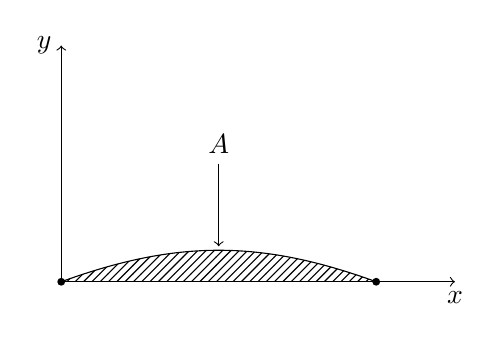
\begin{tikzpicture}[x=4cm,y=3cm]
    \draw[<-] (0,1)node[left]{$y$} -- (0,0);
    \draw[->] (0,0) -- (1.25,0)node[below]{$x$};
    \draw (0,0)node[circle,fill,inner sep=1pt]{};
    \draw (1,0)node[circle,fill,inner sep=1pt]{};
    \draw[pattern=north east lines] (0,0) to[out=20,in=160] (1,0){};
    \draw[->] (0.5,0.5)node[above]{$A$} -- (0.5,0.15);
  \end{tikzpicture}
  \caption{}
  \label{fig:4.6.5}
\end{figure}
\subsubsection*{Remarks}
Find extremals for $F(y)=\int_0^1\sqrt{1+{(y')}^2}\dd{x}$ subject to
$G(y)=\int_0^1y\;\dd{x}=A$ where $y(0)=0$ and $y(1)=0$. For concreteness, assume
$A=\pi/16$. What happens if $A>\pi/8$?
\subsubsection*{Solution}
\todo{}

\section{Mini-lab}
When its ends are attached to two fixed points, a chain of given length and
weight will hang to form a suspension curve. The resulting shape can be
described as that curve $y(x)$, $x\in[-L,L]$ which minimizes the chain
potential energy $E(y)$ subject to the length condition $G(y)=\ell$ where
\begin{equation}
  \label{eq:minilab-problem}
  E(y) = \int_{-L}^{L}\rho g y(x)\sqrt{1+{[y'(x)]}^2\;\dd{x}},\quad
  G(y)=\int_{-L}^{L}\sqrt{1+{[y'(x)]}^2\;\dd{x}}.
\end{equation}
In the above, $\ell$ is the chain length, $\rho$ is the chain mass per unit
length, and $g$ is gravitational acceleration. Here we find candidates for local
minimizers in the $C^2$-norm in the space $V-\{y\in
C^2[-L,L]\;|\;y(-L)=0,\;y(L)=0\}$. We assume $\rho$, $g$, $\ell$, and $L$ are
given positive constants.

\subsection{}
\subsubsection*{Problem}
\label{sec:minilab-a}
Write out the boundary-value problem that any candidate curve $y\in V$ must
satisfy, and find the general solution of the differential equation.

\subsubsection*{Solution}
Let
\begin{align*}
  L &= \rho g y \sqrt{1+{[y'(x)]}^2} \\
  M &= \sqrt{1+{[y'(x)]}^2} \\
  N &= L + \lambda N \\
    &= \rho g y(x)\sqrt{1+{[y'(x)]}^2} + \sqrt{1+{[y'(x)]}^2} \\
  N_{y'} &= \frac{(\rho g y(x) + \lambda) y'(x)}{\sqrt{1+{[y'(x)]}^2}} \\
\end{align*}
The Euler equation turns out to be
\begin{align*}
  c &= N - y'(x)N_{y'} \\
    &= (\rho g y(x) + \lambda)\sqrt{1+{[y'(x)]}^2} -
      \frac{{[y'(x)]}^2(\rho g y(x) + \lambda)}{\sqrt{1+{[y'(x)]}^2}} \\
\end{align*}
From this result we may obtain a relation for ${[y'(x)]}^2$.
\begin{equation}
  \label{eq:minilab-a-yps}
  {[y'(x)]}^2 = \frac{{(\rho g y(x) + \lambda)}^2}{c^2} - 1
\end{equation}
Let $za = \rho g y(x) + \lambda$. Thus
\begin{align*}
  az(x) &= \rho g y(x) + \lambda \\
  \implies y(x) &= \frac{az(x)}{\rho g} - \frac{\lambda}{\rho g} \\
  \implies y'(x) &= \frac{a}{\rho g} \od{z}{x}.
\end{align*}
Now we may rewrite \cref{eq:minilab-a-yps} in terms of $z(x)$.
\begin{align*}
  \frac{a^2}{\rho^2g^2}{\left( \od{z}{x} \right)}^2
  &= \frac{z^2\cancel{a^2}}{\cancel{a^2}} - 1 \\
  \od{z}{x} &= \frac{\rho g }{a}\sqrt{z^2-1} \\
\end{align*}
We may solve this ODE by standard methods.
\begin{equation}
  \label{eq:minilab-b-z}
  \begin{aligned}
    z(x) &= \frac{e^{-\frac{\rho g x}{a}-d} + e^{\frac{\rho g x}{a}+d}}{2} \\
    &= \cosh\left(\frac{\rho g x}{a} + d\right)
  \end{aligned}
\end{equation}
Rewriting \cref{eq:minilab-b-z} in terms of $y(x)$ gives us the general
solution.
\begin{equation*}
  \boxed{y(x) = \frac{a}{\rho g}\cosh\left(\frac{\rho g x}{a}+d\right) - \frac{\lambda}{\rho g}}
\end{equation*}

\subsection{}
\subsubsection*{Problem}
By relabeling constants as necessary, show that the conditions $y(-L)=0$,
$y(L)=0$, and $G(y)=\ell$ can be reduced to two equations for two unknown
constants $b$ and $c$; specifically
\begin{equation}
  \label{eq:minilab-b-problem}
  \frac{bc}{L}=\cosh(c),\quad \frac{\ell c}{2L}=\sinh(c)
\end{equation}

\subsubsection*{Solution}
$y(-L)=0$ and $y(L)=0$ implies that
\begin{equation*}
  \begin{aligned}
    \frac{a}{\rho g}\cosh\left(\frac{\rho g L}{a}+d\right) - \frac{\lambda}{\rho g}
    &= \frac{a}{\rho g}\cosh\left(-\frac{\rho g L}{a}+d\right) - \frac{\lambda}{\rho g} \\
    \frac{a}{\rho g}\cosh\left(\frac{\rho g L}{a}+d\right)
    &= \frac{a}{\rho g}\cosh\left(-\frac{\rho g L}{a}+d\right) \\
    \cosh\left(\frac{\rho g L}{a}+d\right) &= \cosh\left(-\frac{\rho g L}{a}+d\right).
  \end{aligned}
\end{equation*}
Since $\cosh$ is symmetric, $\implies d=0$.
\begin{align*}
  \therefore \; y(x) &= \frac{a}{\rho g}\cosh\left(\frac{\rho g x}{a}\right)
  - \frac{\lambda}{\rho g},\\
  y'(x) &= \sinh\left(\frac{\rho g x}{a}\right).
\end{align*}
We'll invoke the length condition $G(y)=\ell$:
\begin{align*}
  \ell
  &= \int_{-L}^L \sqrt{1 + {\left[ \sinh\left(\frac{\rho g x}{a}\right) \right]}^2} \dd{x} \\
  &= \int_{-L}^L \cosh\left(\frac{\rho g x}{a}\right) \dd{x} \\
  &= \left[ \frac{a}{\rho g}\sinh\left( \frac{\rho g x}{a} \right) \right]_{-L}^{L} \\
  &= \frac{2a}{\rho g}\sinh\left( \frac{\rho g L}{a} \right) \\
\end{align*}
Let $c = \frac{\rho g L}{a}$. Then
\begin{equation*}
  \boxed{\frac{\ell c}{2L} = \sinh(c)}
\end{equation*}
For $y(L)=0$, we have
\begin{align*}
  y(L) &= \frac{a}{\rho g}\cosh\left(\frac{\rho g L}{a}\right) - \frac{\lambda}{\rho g} \\
  0 &= \frac{a}{\rho g}\cosh\left(\frac{\rho g L}{a}\right) - \frac{\lambda}{\rho g} \\
  \frac{\lambda}{\rho g} &= \frac{a}{\rho g}\cosh\left(\frac{\rho g L}{a}\right) \\
  \frac{\lambda}{a} &= \cosh\left( \frac{\rho g L}{a} \right) \\
  \frac{\lambda}{a} &= \cosh(c) \\
\end{align*}
Let $b = \frac{\rho g L}{a}$. Thus
\begin{equation*}
  \boxed{\frac{bc}{L}=\cosh(c).}
\end{equation*}

\subsection{}
\subsubsection*{Problem}
Show that \cref{sec:minilab-a} has two solutions for the pair $b$, $c$ if
$\ell/(2L)>1$, and no solution if $0<\ell/(2L)<1$. Hence we have two or no
candidate curves depending on the ratio $\ell/(2L)$. What happens if
$\ell/(2L)=1$? What is the only possible shape of the suspension curve in this
case? What is the physical reason there can be no solution if $0<\ell/(2L)<1$?

\subsubsection*{Solution}
\todo{}

\subsection{}
\subsubsection*{Problem}
In the case when $ell/(2L)>1$ and there are two candidate curves, it can be
shown that one is a local minimizer and the other a local maximizer. Find and
make plots of these curves for the case of a chain of length $\ell=0.5\text{m}$
of mass $m-0.005\text{kg}$ (so $\rho=m/\ell$) suspended between points with
separation $2L=0.2\text{m}$, where $g=9.8\text{m/s$^2$}$. Indicate which is the
minimizer and maximizer; this should be clear. What is the middle sag-depth
$q=|y(0)|$ for the energy-minimizing shape?

\subsubsection*{Solution}
\todo{}

\end{document}
